\documentclass[12pt]{article}

\usepackage[utf8]{inputenc} 
\usepackage[serbian]{babel}
\usepackage{amsmath}  
\usepackage{amsfonts}
\usepackage{amssymb}
\usepackage{graphicx}
\usepackage{hyperref}
\usepackage{xcolor}
\usepackage{geometry}
\usepackage{algorithm}
\usepackage{algorithmic}
\usepackage{subcaption}
\geometry{a4paper, margin=1in}

\title{Genetski algoritam sa nedominiranim sortiranjem (NSGA-II) \\
\normalsize Seminarski rad u okviru kursa\\ Računarska inteligencija
\\Matematički fakultet}
\author{Staša Đorđević}
\date{\today} 

\begin{document}

\maketitle

\tableofcontents

\section{Uvod u genetske algoritme}
Genetski algoritmi predstavljaju grupu optimizacionih metoda koje se zasnivaju na principima prirodne selekcije i evolucije. Inspirisani su biološkim procesima kao što su selekcija, ukrštanje (kroz reprodukciju), mutacija i nasleđivanje, koji omogućavaju preživljavanje i adaptaciju organizama u prirodi. Slično tome, osnovni koraci u implementaciji genetskih algoritama uključuju selekciju, ukrštanje i mutaciju. Ovi koraci se ponavljaju kroz više generacija kako bi se iz populacije rešenja razvila najbolja moguća rešenja za dati problem.

\begin{itemize}
    \item \textbf{Selekcija} je proces odabira jedinki za ukrštanje na osnovu njihove prilagođenosti. Postoje dve osnovne varijante selekcije:
    \begin{enumerate}
        \item \textbf{Turnirska selekcija} - Odabir k slučajnih jedinki iz populacija i "turnirsko takmičenje" gde pobeđuje najprilagođenija od izabranih jedinki
        \item \textbf{Ruletska selekcija} - U ovoj metodi, verovatnoća selekcije jedinke zavisi od njene uspešnosti u odnosu na ostale jedinke u populaciji. Prilagođenije jedinke imaju veću verovatnoću da budu izabrane, slično kao u ruletu.
    \end{enumerate}
    \item \textbf{Ukrštenje} omogućava kombinovanje gena odabranih jedinki, stvarajući nove potomke koji mogu naslediti najbolje karakteristike svojih "roditelja". Postoji nekoliko osnovnih varijanti ukrštanja:
    \begin{enumerate}
        \item \textbf{Jednopoziciono ukrštanje} - Genetski materijal od roditelja se deli na osnovu jedne slučajno odabrane tačke preseka, a potomci nasleđuju deo od oba roditelja prema toj tački.
        \item \textbf{Višepoziciono ukrštanje} - Ova metoda koristi više tačaka preseka na genomima roditelja, što omogućava veću raznovrsnost u potomcima.
        \item \textbf{Uniformno ukrštanje} - U ovoj varijanti, gene sa oba roditelja se nasumično kombinuju kako bi se stvorio potomak, bez fiksnih tačaka preseka.
    \end{enumerate}
    \item \textbf{Mutacija} se koristi da bi se unela nasumična promena u genetski kod jedinke, što omogućava istraživanje novih mogućnosti i sprečava algoritam da se 'zaglavi' u lokalnim ekstemumima.
\end{itemize}

\textbf{Elitizam} je metoda koja garantuje da će najbolje jedinke iz trenutne generacije biti prenete u sledeću generaciju bez promena. Elitizam se koristi kako bi se sprečilo da se najbolja rešenja izgube tokom evolucije.

Kroz ove procese, genetski algoritmi omogućavaju efikasno istraživanje prostora rešenja i postepeno poboljšanje kvaliteta rešenja tokom vremena.

\section{Opis algoritma NSGA-II}
Algoritam NSGA-II (Non-dominated Sorting Genetic Algorithm II)  je popularan genetski algoritam zasnovan na nedominaciji za višeciljnu optimizaciju. Njegova modifikovana verzija, NSGA-II, koja rešava neke probleme zbog kojih je kritikovana osnovna verzija algoritma, često se koristi kao efikasnije rešenje u primenama višeciljne optimizacije.
Višeciljna optimizacija podrazumeva istovremenu optimizaciju dva ili više međusobno suprostavljenih ciljeva. Cilj je naći skup rešenja koji je najbolji kompromis između ciljeva. Ta rešenja formiraju tzv. \textbf{Pareto front}, u kojem nijedno rešenje nije bolje od drugog, osim ako se jedan cilj ne poboljša na račun pogoršanja drugog.

U NSGA-II algoritmu, termini \textit{non-dominated} i \textit{dominated} se koriste da opišu odnos između rešenja na osnovu njihovih performansi u odnosu na više ciljeva optimizacije.

Rešenje se smatra \textbf{nedominiranim} (engl. \textit{non-dominated}) u odnosu na drugo rešenje ako nijedno od njih nije bolje u svim ciljevima. Drugim rečima, rešenje \(A\) je \textit{nedominirano} u odnosu na rešenje \(B\) ako:

\begin{itemize}
    \item \(A\) nije lošije u svim ciljevima od \(B\),
    \item i \(B\) nije lošije u svim ciljevima od \(A\).
\end{itemize}

Rešenje se smatra \textbf{dominiranim} (engl. \textit{dominated}) u odnosu na drugo rešenje ako postoji rešenje koje je bolje u svim ciljevima. Drugim rečima, rešenje \(A\) je \textit{dominirano} u odnosu na rešenje \(B\) ako:

\begin{itemize}
    \item \(B\) je bolje ili jednako u svim ciljevima od \(A\),
    \item i u barem jednom cilju \(B\) je bolje od \(A\).
\end{itemize}

Kratak opis algoritma:
Prvo se populacija inicijalizuje na standardan način, u skladu sa problemom koji rešavamo. Nakon toga, jedinke u njoj se sortiraju po frontovima prema principu nedominacije. Prvi front je potpuno nedominirani skup u trenutnoj populaciji, tj. skup svih rešenja od kojih ne postoji bolje rešenje u svim ciljevima. Drugi front sadrži jedinke koje su dominirane samo od strane jedinki iz prvog fronta, i tako dalje. Svakoj jedinki se dodeljuje rang na osnovu fronta kojem pripadaju - one iz prvog fronta dobijaju rang 1, iz drugog 2, i tako dalje.
Pored ranga, svaka jedinka ima i novi parametar - \textit{distanca gužve} (engl. \textit{crowding distance}). To je mera koja se koristi za održavanje raznolikosti između rešenja unutar jednog pareto fronta. Predstavlja meru bliskosti jedinke njenim susedima. Veća prosečna distanca gužve rezultira boljom raznovrsnošću u populaciji. Favorizuje manje naseljene regione. Nakon sortiranja, unutar svakog fronta, računa se distanca gužve za jedinke u tom frontu.
Primarni kriterijum za selekciju je rang. Ako dve jedinke imaju isti rang, bolja je ona sa većom distancom gužve.
Ovaj pristup osigurava da algoritam održava i intenzifikaciju (kroz rang) i diverzifikaciju (kroz distancu gužve).
Roditelji se biraju iz populacije koristeći turnirsku selekciju. Odabrana populacija generiše potomke pomoću operacija ukrštanja i mutacije, koje će biti detaljnije opisane u narednom poglavlju.
Populacija, zajedno sa trenutnom populacijom i trenutnim potomcima, ponovo se sortira prema principu nedominacije, i samo se najboljih N jedinki selektuje, gde je N veličina populacije. Selekcija se zasniva na rangu i distanci gužve u poslednjem pareto frontu.

\section{Opis mog rešenja}
\subsection{Grupisanje u pareto frontove - sortiranje}
Ovaj algoritam koristi metod nedominiranog sortiranja da bi organizovao populaciju u Pareto frontove. U prvom koraku se inicijalizuje broj dominacija i lista dominiranih jedinki za svaku jedinku. Zatim, kroz dvostruki for petlju, algoritam poredi svaku jedinku sa svim ostalim u populaciji i ažurira broj dominacija i listu dominiranih jedinki. Nakon što su svi odnosi dominacije utvrđeni, jedinke se grupišu u Pareto frontove prema njihovoj dominaciji. Nakon što je jedinka pridružena određenom Pareto frontu, dodeljuje joj se rang na osnovu njega, koji će nam kasnije koristiti u selekciji.


\begin{algorithmic}[1]
\STATE \textbf{Input:} populacija
\STATE \textbf{Output:} pareto frontovi
\STATE pareto frontovi $\gets$ prazna lista
\STATE broj dominacija $\gets$ prazna mapa
\STATE dominirane jedinke $\gets$ prazna mapa
\STATE n $\gets$ dužina populacije

\FOR{svaku jedinku u populaciji}
    \STATE broj dominacija[jedinka] $\gets$ 0
    \STATE dominirane jedinke[jedinka] $\gets$ prazna lista
\ENDFOR

\FOR{i = 0 \textbf{to} n-1}
    \FOR{j = 0 \textbf{to} n-1}
        \IF{i $\neq$ j}
            \IF{dominira(populacija[i], populacija[j])}
                \STATE dodaj populacija[j] u dominirane jedinke[populacija[i]]
            \ELSIF{dominira(populacija[j], populacija[i])}
                \STATE broj dominacija[populacija[i]] $\gets$ broj dominacija[populacija[i]] + 1
            \ENDIF
        \ENDIF
    \ENDFOR
\ENDFOR

\STATE trenutni front $\gets$ sve jedinke sa brojem dominacija 0
\STATE trenutni indeks $\gets$ 1

\WHILE{trenutni front nije prazan}
    \STATE dodaj trenutni front u pareto frontovi
    \STATE sledeći front $\gets$ prazna lista

    \FOR{svaku jedinku u trenutnom frontu}
        \STATE rang jedinke $\gets$ trenutni indeks
        \FOR{svaku dominiranu jedinku}
            \STATE broj dominacija[dominirana] $\gets$ broj dominacija[dominirana] - 1
            \IF{broj dominacija[dominirana] == 0}
                \STATE dodaj dominiranu u sledeći front
            \ENDIF
        \ENDFOR
    \ENDFOR

    \STATE trenutni front $\gets$ sledeći front
    \STATE trenutni indeks $\gets$ trenutni indeks + 1
\ENDWHILE

\RETURN pareto frontovi
\end{algorithmic}


\subsection{Određivanje distance gužve}
Ova funkcija izračunava distancu gužve za svaku jedinku u Pareto frontu, koristeći sve ciljeve optimizacije. Za svaku jedinku u Pareto frontu, vrednost distance gužve se inicijalizuje na 0. Zatim se za svaki cilj, Pareto front sortira prema vrednostima cilja, a prvoj i poslednjoj jedinki dodeljuje se beskonačna vrednost distance gužve. Distanca za svaku jedinku i svaki cilj se izračunava kao odnos razlike između fitnesa susednih jedinki i razlike između minimalne i maksimalne vrednosti fitnesa (unutar trenutnog Pareto fronta) za dati cilj. Izračunata distanca se dodaje na ukupnu distancu gužve. Ovaj proces se ponavlja za svaki cilj.

\begin{algorithmic}[1]
\STATE \textbf{Input:} pareto front, broj ciljeva
\STATE \textbf{Output:} ažurirani pareto front sa izračunatim distancama gužve

\STATE n $\gets$ dužina pareto fronta

\FOR{svaka jedinka u pareto frontu}
    \STATE jedinka.distanca gužve $\gets$ 0
\ENDFOR

\FOR{i = 0 \textbf{to} broj ciljeva - 1}
    \STATE sortiraj pareto front prema fitnesu[i]
    \STATE pareto front[first].distanca gužve $\gets$ \(\infty\)
    \STATE pareto front[last].distanca gužve $\gets$ \(\infty\)
    \STATE f\_min $\gets$ pareto front[first].fitness[i]
    \STATE f\_max $\gets$ pareto front[last].fitness[i]

    \FOR{k = 1 \textbf{to} n-2}
        \STATE distanca $\gets$ (pareto front[k+1].fitness[i] - pareto front[k-1].fitness[i]) / (f\_max - f\_min)
        \STATE pareto front[k].distanca gužve $\gets$ pareto front[k].distanca gužve + distanca
    \ENDFOR
\ENDFOR

\RETURN pareto front
\end{algorithmic}

\subsection{Selekcija}
U implementaciji je korišćena turnirsku selekciju. Bira se k nasumičnih jedinki iz populacije, i vraća se najbolja od njih. Kriterijum za određivanje najbolje jedinke je na osnovu ranga - što manji rang - to je bolja jedinka. Ako dve jedinke imaju isti rang, bolja je ona koja ima veću distancu gužve.

\subsection{Ukrštanje}
Zbog testiranja algoritma nad funkcijama koje koriste neprekidne vrednosti, koristimo poseban algoritam ukrštanja: \textbf{SBX} (engl. \textit{Simulated Binary Crossover}). 
Cilj SBX-a je da simulira ponašanje jednodelnog binarnog ukrštanja, ali u prostoru realnih brojeva. Njegova glavna prednost je kontrola stepena intenzifikacije i diverzifikacije kroz \textbf{distributivni indeks ukrštanja} ($\eta_c$). 

SBX generiše dve nove jedinke (potomke) na osnovu dva roditelja, gde vrednosti gena potomaka leže između ili blizu vrednosti gena roditelja. Veća vrednost $\eta_c$ dovodi do stvaranja potomaka bližih roditeljima (podstiče intenzifikaciju), dok manja vrednost omogućava šire istraživanje prostora rešenja (podstiče diverzifikaciju).
Tipične vrednosti za $\eta_c$ su u opsegu od 5 do 20, ali konkretan izbor zavisi od prirode problema i ciljeva optimizacije.

U implementaciji koristimo uniformno ukrštanje - gde se za svaki gen jedinke sa verovatnoćom 0.5 računa nova vrednost gena za potomke koristeći SBX formulu.

\subsubsection*{Koraci algoritma za SBX ukrštanje}
\begin{enumerate}
    \item \textbf{Inicijalizacija i iteracija po genima:}
    \begin{itemize}
        \item Veličina hromozoma ($n$) određuje se kao dužina atributa \texttt{code} roditelja.
        \item Algoritam iterira kroz svaki gen (poziciju) hromozoma.
    \end{itemize}
    
    \item \textbf{Verovatnoća ukrštanja:}
    \begin{itemize}
        \item Sa verovatnoćom 50\% ($random.random() \leq 0.5$), algoritam računa nove vrednosti gena za potomke koristeći SBX formulu.
        \item Ako ukrštanje ne treba da se desi, potomci direktno nasleđuju gene roditelja.
    \end{itemize}
    
    \item \textbf{Računanje parametra $\beta_k$:}
    \begin{itemize}
    	\item $\beta_k$ određuje proporciju ukrštanja
        \item Generiše se uniformni slučajan broj $u \in [0,1]$.
        \item Ako je $u \leq 0.5$, računa se:
        \[
        \beta_k = (2u)^{\frac{1}{\eta_c + 1}}
        \]
        \item Inače, računa se:
        \[
        \beta_k = \left(\frac{1}{2(1-u)}\right)^{\frac{1}{\eta_c + 1}}
        \]
    \end{itemize}
    
    \item \textbf{Generisanje gena za potomke:}
    \begin{itemize}
        \item Koristeći $\beta_k$, potomci nasleđuju kombinacije roditeljskih gena prema sledećim formulama:
        \[
        child1[i] = 0.5 \times ((1 + \beta_k) \times parent1[i] + (1 - \beta_k) \times parent2[i])
        \]
        \[
        child2[i] = 0.5 \times ((1 - \beta_k) \times parent1[i] + (1 + \beta_k) \times parent2[i])
        \]
    \end{itemize}
    
    \item \textbf{Ograničenje vrednosti gena:}
    \begin{itemize}
        \item Osigurava se da svaki gen potomaka ostane u opsegu $[0,1]$ pomoću:
        \[
        child.code[i] = \min(\max(child.code[i], 0), 1)
        \]
    \end{itemize}
\end{enumerate}


\subsection{Mutacija}
U ovom radu koristimo \textbf{polinomijalnu mutaciju} (engl. \textit{Polynomial Mutation}), koja je popularna tehnika u evolutivnim algoritmima za probleme sa realnim vrednostima. Njen cilj je da unese dovoljno varijacije u populaciju kako bi se omogućilo efikasnije pretraživanje prostora rešenja i izbegavanje lokalnih ekstremuma.

Polinomijalna mutacija funkcioniše tako što modifikuje gene jedinke u skladu sa slučajnim brojem $r \in (0,1)$ i distribucionim indeksom mutacije $\eta_m$. Veće vrednosti $\eta_m$ dovode do manjih promena u vrednostima gena, dok manje vrednosti omogućavaju veće promene, čime se podstiče istraživanje šireg prostora rešenja. 

\subsubsection*{Koraci algoritma za polinomijalnu mutaciju}
\begin{enumerate}
    \item \textbf{Iteracija kroz gene jedinke:}
    \begin{itemize}
        \item Algoritam prolazi kroz svaki gen $i$ hromozoma jedinke.
        \item Verovatnoća mutacije za svaki gen je definisana parametrom $p$.
    \end{itemize}

    \item \textbf{Generisanje slučajnog broja $r$:}
    \begin{itemize}
        \item Ako $random.random() < p$, gen se menja.
        \item Generiše se uniformno slučajan broj $r \in (0,1)$.
    \end{itemize}

    \item \textbf{Računanje promene $\Delta_q$:}
    \begin{itemize}
        \item Ako je $r < 0.5$, računa se:
        \[
        \Delta_q = (2r)^{\frac{1}{\eta_m + 1}} - 1
        \]
        \item Ako je $r \geq 0.5$, računa se:
        \[
        \Delta_q = 1 - (2(1 - r))^{\frac{1}{\eta_m + 1}}
        \]
    \end{itemize}

    \item \textbf{Ažuriranje gena:}
    \begin{itemize}
        \item Gen se ažurira dodavanjem $\Delta_q$:
        \[
        child.code[i] \mathrel{+}= \Delta_q
        \]
        \item Osigurava se da gen ostane u opsegu $[0,1]$:
        \[
        child.code[i] = \min(\max(child.code[i], 0), 1)
        \]
    \end{itemize}
\end{enumerate}

Efikasnost polinomijalne mutacije zavisi od pravilnog izbora parametara $p$ i $\eta_m$. U ovom radu koristimo $\eta_m = 20$, što omogućava umeren stepen promene vrednosti gena, dok verovatnoća mutacije $p$ zavisi od specifičnog problema i ciljeva optimizacije.

\subsection{Implementacija algoritma NSGA-II}
Implementacija sledi osnovne korake algoritma opisane u prethodnom delu, uz dodatne detalje vezane za parametre i funkcionalnost. 

\subsubsection*{Parametri funkcije \texttt{nsga2}}
\begin{itemize}
    \item \texttt{population\_size}: Broj jedinki u populaciji.
    \item \texttt{num\_variables}: Broj promenljivih koje definišu svaku jedinku.
    \item \texttt{num\_generations}: Broj generacija (iteracija algoritma).
    \item \texttt{tournament\_size}: Broj jedinki uključenih u turnirsku selekciju.
    \item \texttt{mutation\_prob}: Verovatnoća mutacije za svaki gen jedinke.
    \item \texttt{elitism\_size}: Broj najboljih jedinki koje se direktno prenose u narednu generaciju.
    \item \texttt{objective\_function}: Ciljna funkcija koja se koristi za evaluaciju svake jedinke.
\end{itemize}

\subsubsection*{Opis implementacije}
Algoritam se sastoji od sledećih koraka:
\begin{enumerate}
    \item \textbf{Inicijalizacija populacije:} 
    Početna populacija se generiše nasumično. Svaka jedinka se inicijalizuje sa brojem promenljivih \texttt{num\_variables}, a njena vrednost ciljne funkcije se računa pomoću funkcije \texttt{objective\_function}.
    
    \item \textbf{Sortiranje prema dominaciji:} 
    Na početku svake iteracije populacija se sortira u Pareto frontove koristeći funkciju \texttt{non\_dominated\_sorting}. Svakom frontu se dodeljuje rang, a jedinkama unutar frontova računa se distanca gužve (\textit{crowding distance}) radi održavanja raznovrsnosti rešenja.
    
    \item \textbf{Elitizam:} 
    Najboljih \texttt{elitism\_size} jedinki prenosi se direktno u sledeću generaciju. Ovaj pristup osigurava očuvanje najboljih rešenja tokom evolucije.
    
    \item \textbf{Selekcija roditelja:} 
    Roditelji se biraju korišćenjem turnirske selekcije, gde su jedinke sa manjim rangom i većom distancom gužve preferirane. Ovo osigurava da se favorizuju kvalitetna i raznovrsna rešenja.
    
    \item \textbf{Generisanje potomaka:} 
    Nad izabranim roditeljima se primenjuje ukrštanje i polinomijalna mutacija kako bi se generisale nove jedinke. Mutacija se primenjuje sa verovatnoćom \texttt{mutation\_prob}.
    
    \item \textbf{Ažuriranje populacije:} 
    Kombinovanjem trenutne populacije i potomaka kreira se nova populacija veličine \texttt{population\_size}. Selekcija novih jedinki se vrši na osnovu ranga i distance gužve.
    
    \item \textbf{Vizualizacija rezultata:} 
    Nakon završetka iteracija, krajnji Pareto front se prikazuje grafički kako bi se vizualizovala raspodela rešenja.
\end{enumerate}

\section{Eksperimentalni rezultati}
U ovoj sekciji su predstavljeni rezultati NSGA-II algoritma za ciljne funkcije \( ZDT1 \), \( ZDT2 \), i \( ZDT3 \). Ove funkcije su standardni benchmark testovi u višeciljnoj optimizaciji.

\subsection{Opis ciljnih funkcija}
\subsubsection*{ZDT1}
Pareto front ove funkcije je konveksan, što je čini jednostavnom za optimizaciju. Glavni cilj je testiranje sposobnosti algoritma da pronađe ravnomerno raspodeljena rešenja na frontu.
\[
\begin{aligned}
    f_1(x) &= x_1, \\
    f_2(x) &= g(x) \cdot \left(1 - \sqrt{\frac{f_1(x)}{g(x)}}\right),
\end{aligned}
\]
gde je:
\[
g(x) = 1 + \frac{9}{n-1} \sum_{i=2}^n x_i,
\]
i \( x_1 \in [0, 1] \), \( x_i \in [0, 1] \) za \( i = 2, 3, \dots, n \).
\[\]

\subsubsection*{ZDT2}
Ova funkcija ima konkavan Pareto front, što je izazovnije u poređenju sa ZDT1.
\[
\begin{aligned}
    f_1(x) &= x_1, \\
    f_2(x) &= g(x) \cdot \left(1 - \left(\frac{f_1(x)}{g(x)}\right)^2\right),
\end{aligned}
\]
gde je:
\[
g(x) = 1 + \frac{9}{n-1} \sum_{i=2}^n x_i,
\]
i \( x_1 \in [0, 1] \), \( x_i \in [0, 1] \) za \( i = 2, 3, \dots, n \).

\subsubsection*{ZDT3}
Pareto front je isprekidan i sastoji se od više nepovezanih delova, što predstavlja dodatni izazov za algoritam u održavanju raznovrsnosti.
\[
\begin{aligned}
    f_1(x) &= x_1, \\
    f_2(x) &= g(x) \cdot \left(1 - \sqrt{\frac{f_1(x)}{g(x)}} - \frac{f_1(x)}{g(x)} \cdot \sin(10\pi f_1(x))\right),
\end{aligned}
\]
gde je:
\[
g(x) = 1 + \frac{9}{n-1} \sum_{i=2}^n x_i,
\]
i \( x_1 \in [0, 1] \), \( x_i \in [0, 1] \) za \( i = 2, 3, \dots, n \).

\section{Poređenje mojih rezultata i onih iz literature}

\subsection{Pymoo}
Pymoo je optimizaciona biblioteka razvijena u Pythonu, namenjena rešavanju višekriterijumskih optimizacionih problema. Njena implementacija NSGA-II algoritma je dobro optimizovana i široko korišćena u istraživačkim radovima i industrijskim primenama.
Za poređenje mog rešenja sa rešenjem iz biblioteke pymoo, koristiću nekoliko metrika koje omogućavaju objektivnu procenu kvaliteta rešenja:
\begin{enumerate} 
	\item {Hipervolumen (HV)} 
	\item {Maksimalni raspon (MS)}  
	\item {Uniformnost distribucije rešenja} 
\end{enumerate}
\
U literaturi \cite{gete-plots} algoritam se testirao sa sledećim parametrima:
\begin{itemize}
\item veličina populacije = 100
\item broj generacija = 200 za HV i raspodelu, 300 za MS
\item ukrštanje - dvopoziciono
\item verovatnoća ukrštanja = 0.9
\item mutacija - polinomijalna
\item verovatnoća mutacije = 0.033
\item referentna tačka = (1.2, 1.5)
\end{itemize}
U našem rešenju, koristićemo iste parametre tamo gde mogu da budu isti.
\\
Nakon isprobavanja, došla sam do zaključka da je bolje povećati broj generacija. Primetila sam mnogo veća odstupanja kad sam inicijalno stavila da je broj generacija 200. Kada sam promenila da broj generacija bude 500, dobila sam značajno bolje rezultate. Time zaključujem da pymoo algoritam brže konvergira od moje implementacije algoritma.

\subsubsection{Hipervolumen (HV)}
Hipervolumen meri oblast pokrivenu rešenjima na Pareto frontu u višedimenzionalnom prostoru. Za dva cilja, to je površina između tačaka na Pareto frontu i referentne tačke, koja se nalazi izvan dometa svih rešenja, često sa većim vrednostima nego što je moguće dostići.
   
Formule za izračunavanje hipervolumena su sledeće:

- Površina između dve uzastopne tačke na Pareto frontu:
  \[
  \text{Površina} = \text{Širina} \times \text{Visina}
  \]
  gde je širina razlika između vrednosti prvog cilja (\( f_1 \)) dve tačke, a visina je prosečna visina između vrednosti drugog cilja (\( f_2 \)).

- Površina između poslednje tačke i referentne tačke:
  \[
  \text{Površina poslednje} = (r_1 - f_1) \times (r_2 - f_2)
  \]
  gde su \( f_1 \) i \( f_2 \) koordinate poslednje tačke na Pareto frontu, a \( r_1 \) i \( r_2 \) su vrednosti referentne tačke.

Rezultati hipervolumena nam omogućavaju da procenimo efikasnost i uniformnost distribucije rešenja na Pareto frontu. Veći hipervolumen ukazuje na bolji raspored rešenja i bolju pokrivenost prostora ciljeva.

\begin{figure}[H]
    \centering
    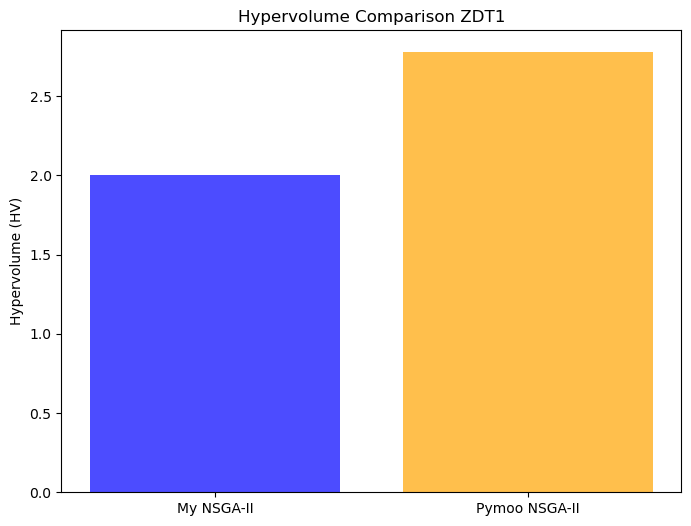
\includegraphics[width=0.7\textwidth]{images/hv_zdt1.png}
    \caption{Poređenje hipervolumena za \( ZDT1 \) funkciju.}
    \label{fig:hv_zdt1}
\end{figure}

\begin{figure}[H]
    \centering
    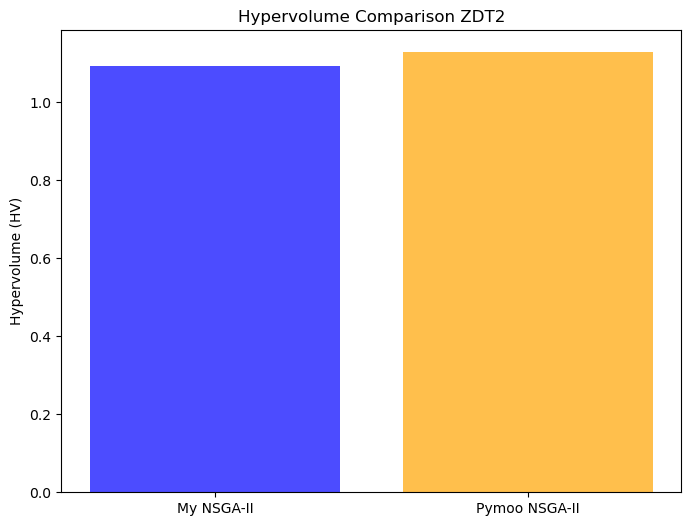
\includegraphics[width=0.7\textwidth]{images/hv_zdt2.png}
    \caption{Poređenje hipervolumena za \( ZDT2 \) funkciju.}
    \label{fig:hv_zdt2}
\end{figure}

\begin{figure}[H]
    \centering
    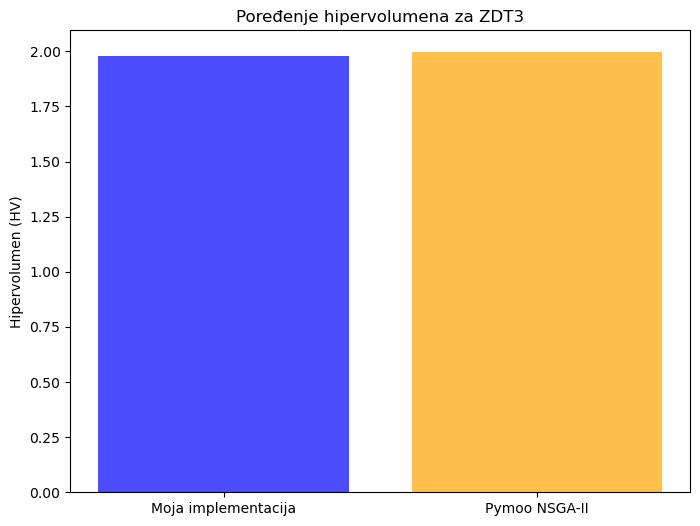
\includegraphics[width=0.7\textwidth]{images/hv_zdt3.png}
    \caption{Poređenje hipervolumena za \( ZDT3 \) funkciju.}
    \label{fig:hv_zdt3}
\end{figure}

U poređenju hipervolumena između moje implementacije NSGA-II i pymoo implementacije, rezultati pokazuju gotovo identične vrednosti, s tim da je moj hipervolumen za veoma malu vrednost manji u svim testiranim funkcijama, što je i očekivano. To ukazuje na to da je moj algoritam uspešno postigao visok nivo pokrivanja prostora ciljeva, odnosno da je Pareto front ravnomerno raspoređen i da su rešenja dobar odraz kvaliteta.

\subsubsection{Maksimalni raspon (MS)}
Maksimalni raspon (engl. \textit{maximal spread}) meri udaljenost između najudaljenijih tačaka na Pareto frontu po svakom cilju. Ovo nam daje uvid u to kako su rešenja raspoređena duž fronta, tj. koliko je front širok u svakom cilju.
Veća vrednost MS ukazuje na bolju pokrivenost ciljnog prostora, dok manja vrednost može značiti da su rešenja koncentrisana u užem delu fronta.

\begin{figure}[H]
    \centering
    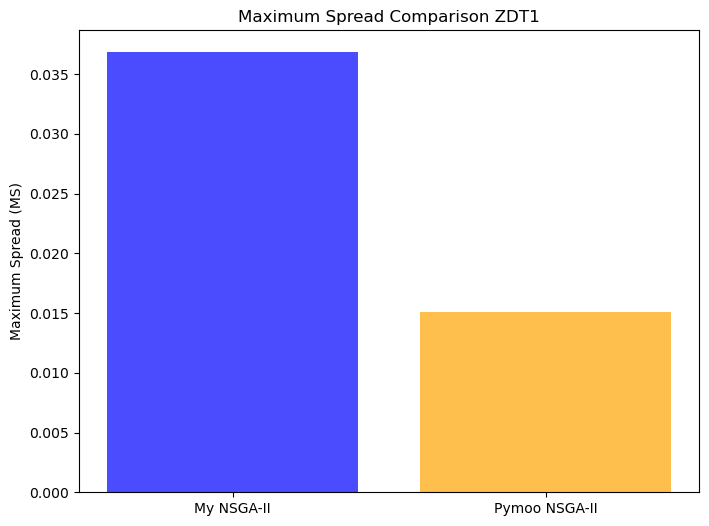
\includegraphics[width=0.7\textwidth]{images/ms_zdt1.png}
    \caption{Poređenje maksimalnog raspona za \( ZDT1 \) funkciju.}
    \label{fig:ms_zdt1}
\end{figure}

\begin{figure}[H]
    \centering
    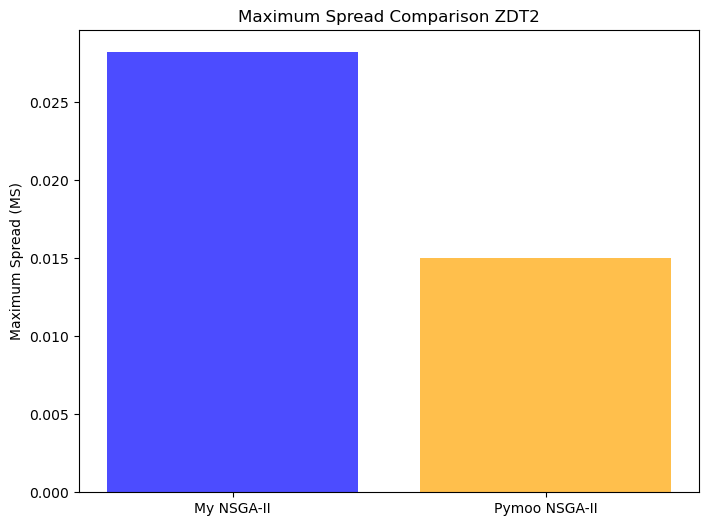
\includegraphics[width=0.7\textwidth]{images/ms_zdt2.png}
    \caption{Poređenje maksimalnog raspona za \( ZDT2 \) funkciju.}
    \label{fig:ms_zdt2}
\end{figure}

\begin{figure}[H]
    \centering
    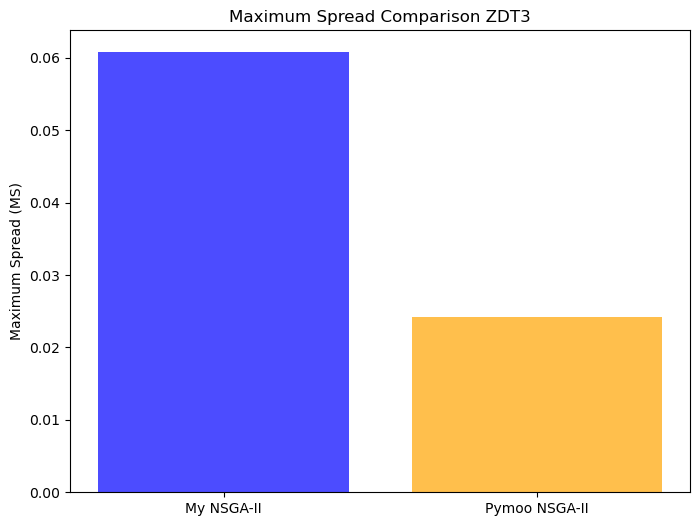
\includegraphics[width=0.7\textwidth]{images/ms_zdt3.png}
    \caption{Poređenje maksimalnog raspona za \( ZDT3 \) funkciju.}
    \label{fig:ms_zdt3}
\end{figure}

Rezultati maksimalnog raspona pokazuju da su vrednosti mog NSGA-II algoritma značajno veće u poređenju sa rezultatima pymoo implementacije.
Ovo sugeriše da su rešenja generisana mojim algoritmom koncentrisanija u širem delu Pareto fronta, što znači da postiže bolju pokrivenost u širini za razliku od pymoo implementacije.

\subsubsection{Uniformnost distribucije rešenja}
Uniformnost distribucije rešenja na Pareto frontu ukazuje na to koliko su tačke ravnomerno raspoređene. Dobar algoritam treba da postigne visok nivo uniformnosti kako bi osigurao kvalitetan i ravnomerno raspoređen Pareto front.

\begin{figure}[H]
    \centering
    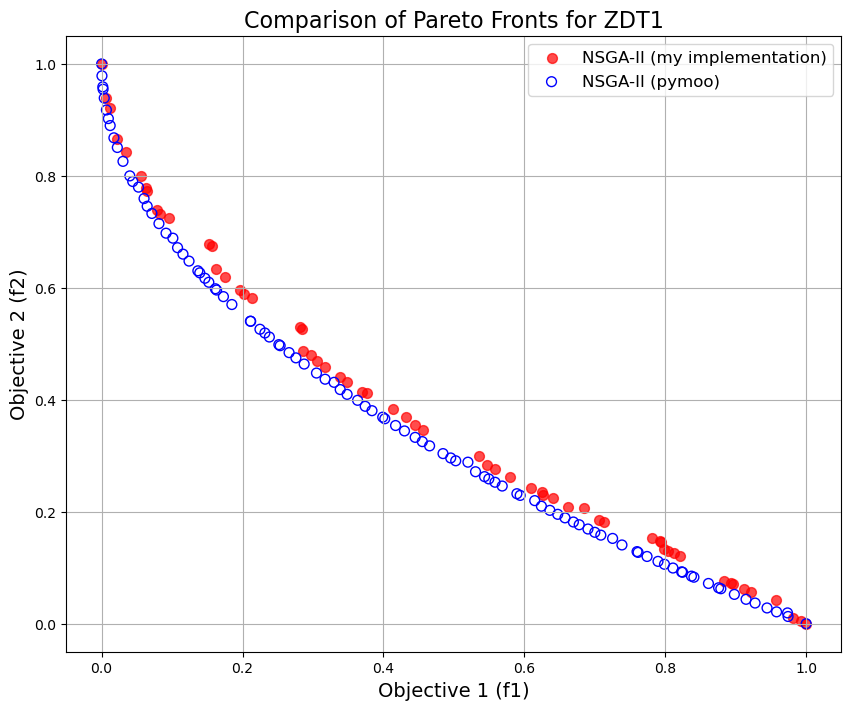
\includegraphics[width=0.7\textwidth]{images/pareto_zdt1.png}
    \caption{Poređenje distribucije rešenja za \( ZDT1 \) funkciju.}
    \label{fig:pareto_zdt1}
\end{figure}

\begin{figure}[H]
    \centering
    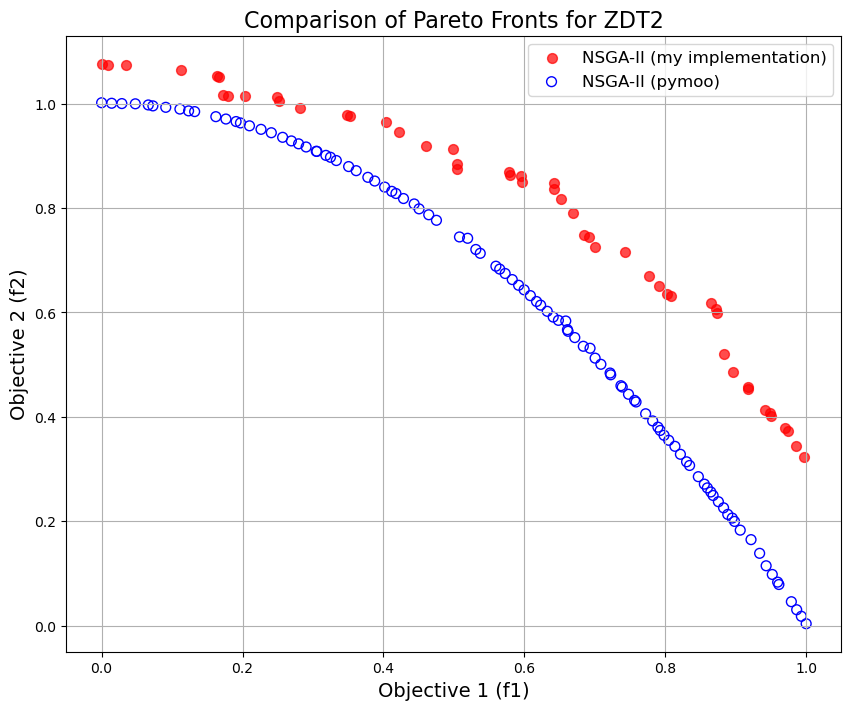
\includegraphics[width=0.7\textwidth]{images/pareto_zdt2.png}
    \caption{Poređenje distribucije rešenja za \( ZDT2 \) funkciju.}
    \label{fig:pareto_zdt2}
\end{figure}

\begin{figure}[H]
    \centering
    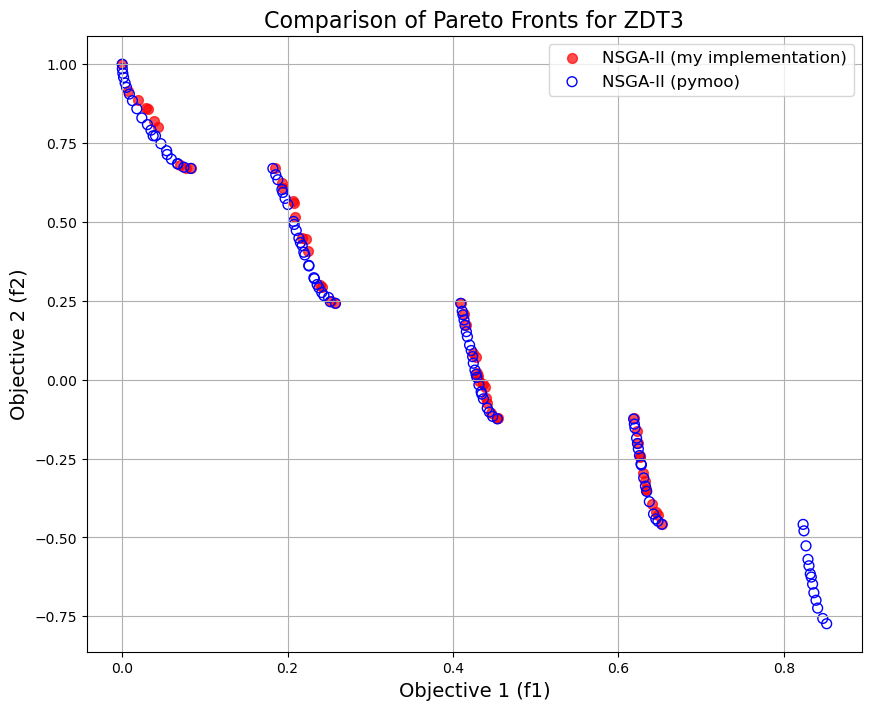
\includegraphics[width=0.7\textwidth]{images/pareto_zdt3.png}
    \caption{Poređenje distribucije rešenja za \( ZDT3 \) funkciju.}
    \label{fig:pareto_zdt3}
\end{figure}

Poređenje uniformnosti distribucije rešenja na Pareto frontu između moje implementacije NSGA-II i pymoo implementacije pokazuje vrlo slične rezultate, sa minimalnim razlikama u distribuciji rešenja. Grafički prikazi pokazuju da se tačke na Pareto frontu vrlo dobro preklapaju, što ukazuje na to da su rešenja ravnomerno raspoređena. Ipak, može se primetiti da su rešenja u mojoj implementaciji nešto manje ravnomerno raspoređena u odnosu na pymoo, ali razlike nisu velike.

\subsection{SPEA2}
Moju implementaciju NSGA2 algoritma uporediću sa još jednim algoritmom koji je namenjen za rešavanje istih problema - u pitanju je \textbf{Evolucioni algoritam sa Pareto snagom 2} (engl. Strenght Pareto Evolutionary Algorithm - SPEA2). 
SPEA2 je evolucioni algoritam za višekriterijumske optimizacione probleme, poboljšana verzija SPEA algoritma. Kao i NSGA-II, koristi Pareto dominaciju za selekciju rešenja, ali uvodi dodatne mehanizme za očuvanje raznovrsnosti populacije. Ključne karakteristike uključuju unapređenu procenu gustine rešenja, eksteran arhiv za skladištenje nedominiranih rešenja i efikasnu strategiju skraćivanja arhiva. Ove osobine omogućavaju SPEA2 algoritmu da bolje aproksimira Pareto front i poboljša stabilnost optimizacije.

Rezultati su veoma slični kao kod poređenja moje implementacije sa bibliotečkom implementacijom NSGA-II algoritma. Na isti način je vršeno poređenje, jer u pymoo biblioteci postoji i SPEA2 algoritam.

Detaljnu implementaciju algortima SPEA2 neću ovde komentarisati, cilj ovog poređenja je samo da se uporedi moja implementacija sa još nekim algoritmom za višekriterijumske optimizacione probleme.

Prikazani su rezultati poređenja za funkciju ZDT2.
\begin{figure}[H]
    \centering
    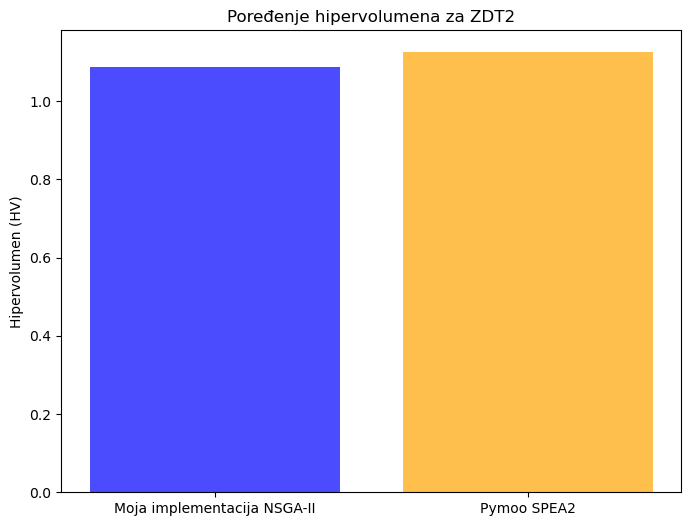
\includegraphics[width=0.7\textwidth]{images/hv_spea2.png}
    \caption{Poređenje hipervolumena za \( ZDT2 \) funkciju.}
    \label{fig:hv_spea2}
\end{figure}

\begin{figure}[H]
    \centering
    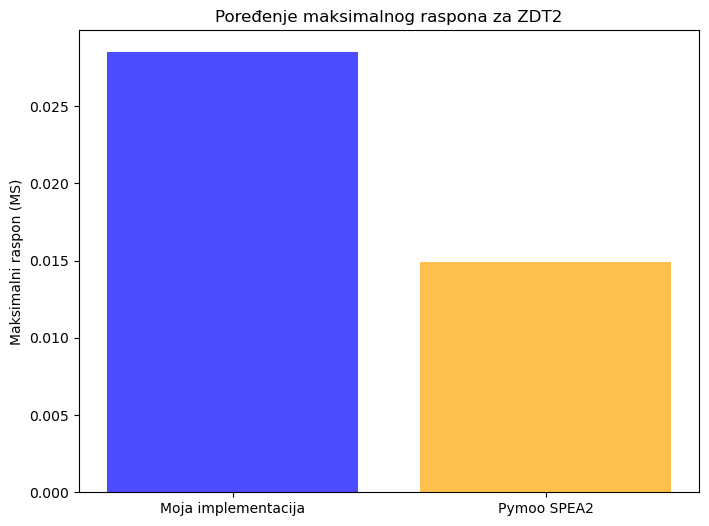
\includegraphics[width=0.7\textwidth]{images/ms_spea2.png}
    \caption{Poređenje maksimalnog raspona za \( ZDT2 \) funkciju.}
    \label{fig:ms_spea2}
\end{figure}

\begin{figure}[H]
    \centering
    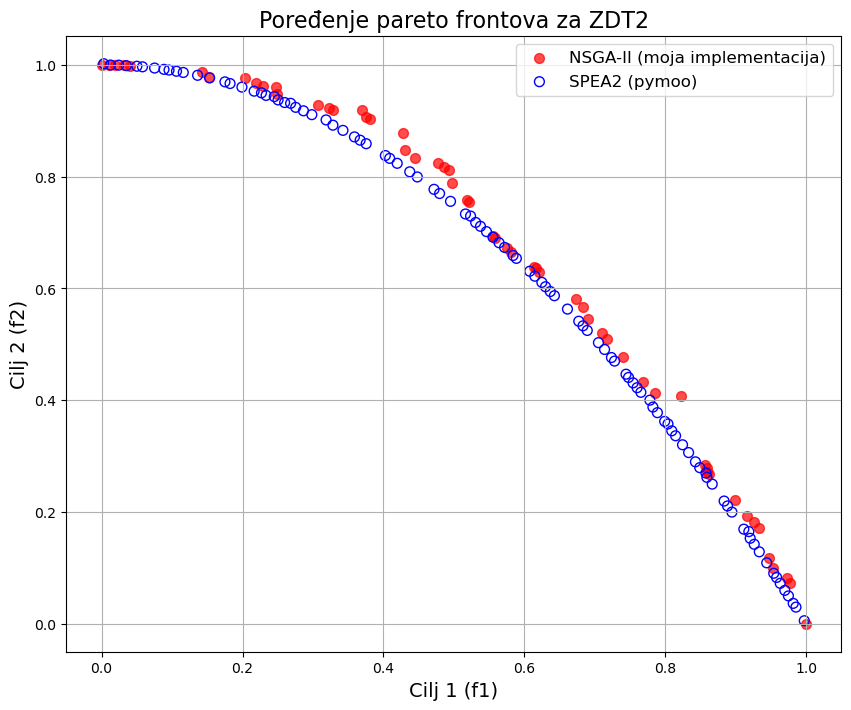
\includegraphics[width=0.7\textwidth]{images/pareto_spea2.png}
    \caption{Poređenje distribucije rešenja za \( ZDT2 \) funkciju.}
    \label{fig:pareto_spea2}
\end{figure}

Primećuju se iste razlike kao kod prethodnog poređenja. SPEA2 u biblioteci pymoo je implementiran tako da daje iste rezultate kao i NSGA-II iz iste biblioteke.


\section{Diskusija o razlikama između implementacija}
Iz prethodne analize, jasno je da postoji određena razlika između moje implementacije i pymoo implementacije NSGA-II algoritma.

Prva značajna razlika odnosi se na proces selekcije i ukrštanja.
Pymoo koristi detaljno podešen operator selekcije roditelja koji omogućava efikasniju genetsku raznovrsnost populacije, dok moja implementacija primenjuje standardnu turnirsku selekciju sa određenom veličinom turnira.  Ova razlika može uticati na način na koji se rešenja raspoređuju duž Pareto fronta, pri čemu pymoo obezbeđuje širu pokrivenost ciljnog prostora, dok moja implementacija može težiti ka centralnim delovima fronta.

Drugi faktor je način na koji se mutacija i ukrštanje sprovode. Obe implementacije koriste polinomijalnu mutaciju, samo što pymoo ima prilagođene distribucione parametre koji omogućavaju bolje balansiranje intenzifikacije i diverzifikacije rešenja, dok moja implementacija koristi fiksne parametre.  Kao rezultat, pymoo može generisati rešenja koja su ravnomernije raspoređena po frontu, dok moja verzija pokazuje značajno veći maksimalni raspon (MS), što znači da obuhvata širu oblast ciljnog prostora. Veći MS u mojoj implementaciji ukazuje da algoritam uspeva da pronađe ekstremne tačke Pareto fronta, ali može dovesti do manje ravnomerne raspodele rešenja, pri čemu neka područja fronta mogu ostati slabije pokrivena.

Treći faktor koji doprinosi razlikama je algoritam sortiranja Pareto fronta. Pymoo implementacija koristi optimizovane procedure za brzo nedominirano sortiranje, koje mogu preciznije obrađivati dominaciju između rešenja i time omogućiti bolju raspodelu tačaka. U mojoj implementaciji, iako se koristi sličan algoritam, moguće su manje razlike u načinu rangiranja i dodeljivanja distance gužve (\textit{crowding distance}), što može dovesti do drugačijeg rasporeda rešenja.

Dodatno, implementacije se razlikuju u brzini konvergencije, tj. efikasnosti. Pymoo implementacija brže postiže stabilne rezultate zbog optimizovanog upravljanja populacijom i mehanizama selekcije, što omogućava efikasnije širenje fronta. U mom slučaju, pokazalo se da povećanje broja generacija značajno poboljšava kvalitet rešenja, što sugeriše da je mojoj implementaciji potrebno više iteracija kako bi dostigla iste nivoe pokrivenosti kao pymoo.

\section{Zaključak}
U ovom radu implementiran je NSGA-II algoritam i upoređen sa postojećom pymoo implementacijom kroz metrike hipervolumena, maksimalnog raspona i uniformnosti distribucije rešenja na Pareto frontu.
Rezultati analize pokazuju da moja implementacija NSGA-II postiže gotovo identične vrednosti hipervolumena kao pymoo implementacija. Ovo potvrđuje da algoritam uspešno generiše kvalitetna rešenja i pokriva relevantan deo prostora ciljeva.

Međutim, maksimalni raspon rešenja u mojoj implementaciji pokazuje značajno više vrednosti u poređenju sa pymoo, što sugeriše da se rešenja nalaze u širem delu Pareto fronta. Veći MS sugeriše da algoritam uspešno pronalazi ekstremne tačke fronta, ali može dovesti do manje ravnomerne raspodele rešenja. Ova razlika može biti posledica parametara selekcije i mutacije.

Jedno od ključnih zapažanja tokom eksperimentisanja jeste da povećanje broja generacija značajno utiče na performanse mog algoritma. Inicijalno sam koristila broj generacija 200, kako je navedeno u literaturi, ali su rezultati pokazali veća odstupanja u odnosu na pymoo implementaciju. Kada sam povećala broj generacija na 500, dobila sam značajno bolje rezultate, što sugeriše da pymoo algoritam brže konvergira u odnosu na moju implementaciju.
\\
\\
Mogući pravci daljeg unapređenja uključuju:

\begin{itemize}
    \item Podešavanje hiperparametara algoritma kako bi se poboljšala širina pokrivenosti Pareto fronta.
    \item Optimizaciju selekcije i mutacije za ravnomerniju distribuciju rešenja.
    \item Istraživanje tehnika ubrzanja konvergencije kako bi algoritam dostizao kvalitetna rešenja u manjem broju generacija.
    \item Proširenje analize na još neke test funkcije i stvarne optimizacione probleme radi bolje procene performansi algoritma.
	\item Prilagođavanje algoritma za rešavanje diskretnih optimizacionih problema.
\end{itemize}

Ova analiza pokazuje da je implementirani NSGA-II algoritam konkurentan u odnosu na pymoo rešenje, ali da postoji prostor za poboljšanja, posebno u pogledu brzine konvergencije i širine pokrivenosti Pareto fronta.

\addcontentsline{toc}{section}{Literatura}
\renewcommand{\refname}{Literatura}
\begin{thebibliography}{10}
\bibliographystyle{unsrt}
\bibitem{ieee} K. Deb, A. Pratap, S. Agarwal and T. Meyarivan, \textit{A fast and elitist multiobjective genetic algorithm: NSGA-II}, \url{https://ieeexplore.ieee.org/abstract/document/996017}

\bibitem{sbx-poly-impl} A. Seshadri, \textit{A fast elitist multiobjective genetic algorithm}, \url{https://www.academia.edu/download/53297141/NSGA_II.pdf}

\bibitem{ri-kurs} Materijali sa kursa \textit{Računarska inteligencija}, Matematički fakultet, Univerzitet u Beogradu

\bibitem{sbx} M. M. N. Rafstedt, \textit{Analyzing the Simulated Binary Crossover Operator in Multi-Objective Evolutionary Algorithms}, \url{https://www.duo.uio.no/handle/10852/111478}

\bibitem{gete-plots} Y. Sato and M. Sato, \textit{Using Dominated Solutions at Edges to the Diversity and the Uniformity of Non‑dominated Solution Distributions in NSGA‑II}, \url{https://www.researchgate.net/publication/362563469_Using_Dominated_Solutions_at_Edges_to_the_Diversity_and_the_Uniformity_of_Non-dominated_Solution_Distributions_in_NSGA-II#fullTextFileContent}

\bibitem{pymoo} pymoo: Multi-objective optimization in Python, \url{https://github.com/anyoptimization/pymoo}

\bibitem{pymoo-calls} \url{https://pymoo.org/algorithms/moo/nsga2.html}

\bibitem{spea2} E. Zitzler, M. Laumanns and L. Thiele, \textit{SPEA2: Improving the Strength Pareto Evolutionary Algorithm}, \url{https://www.research-collection.ethz.ch/handle/20.500.11850/145755}



\end{thebibliography}

\end{document}
